%#!uplatex

\documentclass[a4paper,dvipdfmx,uplatex,twocolumn]{jsarticle} % レジュメ用クラス
\usepackage{style/resume}   % レジュメ用スタイル

% 何も気にせず latexmk でコンパイルするとこの main.tex（レジュメ）がコンパイルされます
% 卒論をコンパイルするときは latexmk thesis.tex のようにファイルを指定しましょう

\begin{document}
    \ThisIsDraft % 下書きの時はこれをつけるとバージョン管理ができます

    
% ----------
\title{卒業研究・卒業制作レジュメのテンプレートと書き方ガイド} % タイトル
\subtitle{} % サブタイトル（必要なければ空にする）

\author{%
    X12345 愛工太郎%
    % \and K11223 愛工二郎  % 複数人いる場合は\andで追加
}

\supervisor{小栗真弥}

% ----------

\maketitle

%% ===========================================================
\section{はじめに}
\label{sec:intro}
本文書は情報科学部の卒業論文・卒業制作要旨集（レジュメ）を執筆するための\upLaTeX 用テンプレートである．
卒業研究（論文）と卒業制作の両方に対応しており，テンプレートの使い方と，レジュメを書く上での注意点をまとめている．
卒業研究では研究の\textbf{新規性}・\textbf{有用性}・\textbf{信頼性}が重視され，卒業制作では作品の\textbf{独自性}・\textbf{メッセージ性}・\textbf{完成度}が重視される．
自分がどちらに該当するかを確認し，該当する部分を参照しながら執筆すること．
\upLaTeX を用いた一般的な文章作成技術については，文献\cite{tex}等を参考にされたい．
レジュメや卒論の執筆には基本的に\upLaTeX の使用を推奨するが，書式が同じであればWordやPages，typstなど，どのようなツールを使っても構わない．
書籍やインターネットで調べると\LaTeX に関する様々な記法やテクニックが簡単に出てくるので，各自で調べながら執筆すること．

%% ===========================================================
\section{テンプレートの使い方}
\label{sec:usage}

\subsection{基本設定}
\label{subsec:basic}
用途に応じてコンパイルの起点となるファイルが異なる．
\begin{itemize}
    \item レジュメ用：\texttt{main.tex}（\texttt{jsarticle}＋\texttt{style/resume}）
    \item 卒論用：\texttt{thesis.tex}（\texttt{jsbook}＋\texttt{style/thesis}）
\end{itemize}
卒論の記述例は\texttt{thesis/example/}にある．
卒論用スタイルは章（\verb|\chapter|）を使うため\texttt{jsbook}クラスが必要であり，\texttt{main.tex}のスタイルだけを差し替えてもコンパイルできない．
卒論をコンパイルするときは\texttt{latexmk thesis.tex}のようにファイル名を指定する．

レジュメの本文の内容は\texttt{resume/}ディレクトリ内の\texttt{.tex}ファイルに記述し，\texttt{main.tex}から\verb|\include{}|で読み込む．
ファイルを分割することで，章ごとの管理がしやすくなる．

\subsection{タイトル・著者情報}
\label{subsec:title}
以下のコマンドでタイトル，著者，指導教員を設定する．
\begin{lstlisting}[language={[LaTeX]TeX}, numbers=none, frame=single]
\title{論文タイトル}
\subtitle{サブタイトル}
\author{X12345 愛工太郎}
\supervisor{指導教員名}
\end{lstlisting}
サブタイトルが不要な場合は\verb|\subtitle|の行を省略すればよい．
著者が複数いる場合は\verb|\and|で繋ぐ．
\begin{lstlisting}[language={[LaTeX]TeX}, numbers=none, frame=single]
\author{X12345 愛工太郎 \and K11223 愛工二郎}
\end{lstlisting}

\subsection{下書きモード}
\label{subsec:draft}
\texttt{main.tex}内で\verb|\ThisIsDraft|を記述すると，ページ左上にビルド日時のバージョン情報が赤字で表示され，ページ上部の中央に「DRAFT」の透かしが入り，ページ番号が付与される．
指導教員への提出時にどの版かを識別するのに便利である．
最終提出時にはこの行を削除またはコメントアウトすること．

\subsection{ビルド方法}
\label{subsec:build}
本テンプレートは\texttt{latexmkrc}にビルド設定が記述されている．
ローカルでコンパイルする場合にはターミナルで以下のコマンドを実行すればPDFが生成される．
\begin{lstlisting}[language=bash, numbers=none, frame=single]
latexmk
\end{lstlisting}
Overleafを使用する場合は，コンパイラをLaTeXに設定し，\texttt{main.tex}をメインファイルに指定する．

%% ===========================================================
\section{レジュメの書き方}
\label{sec:writing}

\subsection{全体の構成}
\label{subsec:structure}
レジュメのタイトルは卒業論文・卒業制作のタイトルと一致させる必要がある．
全体的には5〜6個の節で構成し，必要に応じて小節（subsection）を用いる．
節や全体の構成が不適切な文章は読者にとって大きな負担となる\cite{kisaragi}．

\textbf{卒業研究}の場合の一般的な節構成の例を以下に示す．
\begin{enumerate}
    \item はじめに（研究背景，問題提起，目的，概要）
    \item 関連研究・先行研究
    \item 提案手法
    \item 実験・評価
    \item おわりに（結論，今後の課題）
\end{enumerate}

\textbf{卒業制作}の場合の一般的な節構成の例を以下に示す．
\begin{enumerate}
    \item はじめに（背景・動機，コンセプト，概要）
    \item 作品の特徴（対象者，情動，メッセージ，手法）
    \item 制作内容（設計，実装，技術的工夫）
    \item 制作物の紹介・解説
    \item おわりに（まとめ，今後の展望）
\end{enumerate}
制作の場合には，研究とは異なり主観的な評価に陥りがちである．
そのため作品の対象者を具体的に提示し，メッセージ性としてその対象者に対してどのような情動を引き起こしたいのか，
その情動を引き起こすためにどのような手法をとるのかを明確にすることが重要である．

上記はあくまで一例であり，指導教員の指示に従い，研究・制作の内容に応じて適切な構成を考えること．

\subsection{「はじめに」の書き方}
\label{subsec:intro-writing}
「はじめに」は読者が最初に目にする節であり，レジュメ全体の印象を大きく左右する．

\textbf{卒業研究}の場合は，以下の要素を順に記述するとよい．
\begin{enumerate}
    \item \textbf{研究背景}：その分野の現状や社会的な背景を述べる
    \item \textbf{問題提起}：既存の手法や状況にどのような課題があるかを示す
    \item \textbf{研究目的}：上記の課題に対して本研究が何を目指すかを明確にする
    \item \textbf{研究概要}：目的を達成するためにどのようなアプローチを取ったかを簡潔に述べる
\end{enumerate}

\textbf{卒業制作}の場合は，以下の要素を順に記述するとよい．
\begin{enumerate}
    \item \textbf{制作背景}：制作のきっかけとなった社会的・文化的背景や自身の問題意識を述べる
    \item \textbf{制作動機}：なぜこの作品を制作しようと考えたのか，動機や着想を示す
    \item \textbf{コンセプト}：作品を通じて何を表現・実現しようとしているかを明確にする
    \item \textbf{制作概要}：どのような作品をどのような手法で制作したかを簡潔に述べる
\end{enumerate}

\subsection{「おわりに」の書き方}
\label{subsec:conclusion-writing}
「おわりに」では，本研究・本制作で行ったことと得られた成果を簡潔にまとめる．
「はじめに」で述べた目的に対して，どの程度達成できたかを振り返ることが重要である．
結論が明確でない，範囲や限界の指摘が不適切である，または目的の内容と結論が乖離しているものは再考を要する．

\textbf{卒業研究}の場合は，研究の限界や今後の課題・展望を述べることで，研究の発展性を示す．

\textbf{卒業制作}の場合は，制作を通じて得られた知見や気づき，作品の改善点や今後の発展の可能性について述べる．
当初の制作目的やコンセプトに対して，完成した作品がどの程度それを実現できたかを振り返ることが大切である．

\subsection{文章作成の基本}
\label{subsec:writing-tips}
卒業研究では新規性・有用性・信頼性が，卒業制作では独自性・メッセージ性・完成度が読者に伝わるように記述する\cite{kisaragi}．
読み手にとって読みやすい文章を心がけること．
内容が前後する，背景や課題の設定が不明瞭であるといった文章は読者にとって負担となる．
以下に基本的な注意点をまとめる．
\begin{itemize}
    \item 「だ・である」調（常体）で統一する．「です・ます」調と混在させない
    \item 一文は短く簡潔にする．極端な口語体や長文の連続は避ける
    \item 主語と述語の対応を明確にする．長い文は主述がねじれやすい
    \item 曖昧な表現（「〜と思われる」「〜的な」）を避け，根拠に基づいて断定する
    \item 略語は初出時に正式名称を併記する（例：CNN (Convolutional Neural Network)）
    \item 文中の文脈から推測しないと内容が把握できない論文にしない
    \item 説明に飛躍がないか，逆に冗長すぎる部分がないか確認する
    \item 未定義の用語を減らし，専門用語には適切な説明を付ける
\end{itemize}

\subsection{句読点と文字の使い分け}
\label{subsec:punctuation}
句点には全角の「．」，読点には全角の「，」を用いる（本テンプレートの慣例）．
ただし英文中や数式中で使う場合は半角の「.」「,」を用いる．「。」「、」は使用しない．

全角文字と半角文字の使い分けは以下の通りである．
\begin{itemize}
    \item 英数字，空白，記号類は半角文字を用いる
    \item カタカナは全角文字を用いる
    \item 括弧は全角の「（」「）」を基本とし，英文中では半角の「(」「)」を用いる
    \item 引用符は開きと閉じを区別する．開きには\,``\,を，閉じには\,''\,を用いる
\end{itemize}

\subsection{主張すべきポイント}
\label{subsec:novelty}

\textbf{卒業研究}では，\textbf{新規性}・\textbf{有用性}・\textbf{信頼性}の3点を意識して記述する．
\begin{itemize}
    \item \textbf{新規性}：既知の技術が何であり，何を新しいアイデアとして提案しているのかを明確に書く．提案内容が概念的・抽象的な説明に終始し，読者が具体的な内容を理解できないものは再考を要する
    \item \textbf{有用性}：提案手法がどのような場面で役立つのかを示す．有用性の主張がない，または極めて貧弱なものは再考を要する
    \item \textbf{信頼性}：実験や評価によって主張を裏付ける．実験条件，データの取得方法，評価指標などを明記し，結果の再現性を担保する
\end{itemize}
十分な参考文献の調査と引用は，新規性の主張に欠かせない．

\textbf{卒業制作}では，\textbf{独自性}・\textbf{メッセージ性}・\textbf{完成度}の3点を意識して記述する．
\begin{itemize}
    \item \textbf{独自性}：既存の作品や事例と比較して，自分の作品がどのような点で独自であるかを明確にする．関連作品の調査を行い，それらとの差異を具体的に示すこと
    \item \textbf{メッセージ性}：作品を通じて何を伝えたいのか，どのような体験を提供したいのかを明確に記述する．コンセプトが曖昧なままでは，読者に作品の意図が伝わらない
    \item \textbf{完成度}：作品がどの程度完成しているかを示す．技術的な工夫，デザイン上の判断，試行錯誤の過程などを具体的に記述し，作品の質を読者に伝える
\end{itemize}
卒業制作においても，関連作品や先行事例の調査と引用は独自性の主張に重要である．

\subsection{提出前に他の人に読んでもらう}
\label{subsec:review}
レジュメは必ず提出前に指導教員の確認を受けること．
締切直前にいきなり見せるのではなく，早い段階から計画的に執筆を進め，指導教員からのフィードバックを受けて何度も改良を重ねること．
また，同級生や先輩に読んでもらうことも有効である．
それによって自分では気づかない論理の飛躍や読みにくい箇所を指摘してもらえる．
卒業制作の場合は，作品の意図やコンセプトが文章から正しく伝わるかどうかも確認してもらうとよい．
読者の立場から見て論理的な飛躍がないかに注意して記述すること．

\subsection{生成AIの利用について}
\label{subsec:ai}
ChatGPTやGemini，Claude等の生成AIは，文章の推敲やアイデアの整理など，執筆を補助するツールとして活用できる．
ただし，以下の点に十分注意すること．
\begin{itemize}
    \item 生成AIの出力をそのまま貼り付けてはならない．自分の言葉で書き直したり内容を吟味し自らの文章として記述すること
    \item 生成AIは事実と異なる内容（ハルシネーション）を生成することがあるので出力内容は必ず自分で裏付けを取ること．誤った内容がレジュメに記載された場合，その責任を負うのは生成AIではなく著者自身である
    \item 存在しない参考文献を生成することがあるため，引用情報は必ず原典にあたって確認すること
    \item 生成AIの利用に関する方針は指導教員や学科の指示に従うこと
\end{itemize}
卒業論文・レジュメはあくまで自分自身の研究成果を示すものである．
生成AIはあくまで補助的なツールとして位置づけ，内容の責任は著者自身が負うことを忘れてはならない．

%% ===========================================================
\section{図の使い方}
\label{sec:figure}

図を使用する際は，キャプションを付けるとともに，必ず本文中で図番号を参照すること．
使用していない図を掲載してはならない．
卒業制作の場合は，制作物のスクリーンショットや外観写真など，作品の内容が視覚的に伝わる図を積極的に掲載するとよい．
また，図は自分で作成したものを使用する．
標準テストイメージ等を除き，インターネット等で入手した図や写真をそのまま使ってはならない．
他の論文の図表を引用の明示なく利用することも禁止である．

\subsection{画像形式の選び方}
グラフや線画などのベクター図はPDFまたはEPS形式で用意すると，拡大しても劣化せず印刷品質が高い．
写真やスクリーンショットなどのラスター画像にはPNGやJPEG形式を用いてよい．
レジュメはオフセット印刷で製本されるため，ラスター画像の場合は少なくとも300dpiの解像度を確保すること．
図が不鮮明であったり，大きさや縮尺が不適切であったりするものは再考を要する．

\subsection{図の配置}
\label{subsec:fig-placement}
図の位置指定には\verb|[tb]|を基本とすると読みやすくなる（ページの上部または下部に配置）．
\verb|[h]|で，その場に配置を指示できるが，レイアウトが乱れることがあるので使用には注意をする．
\LaTeX が自動的に適切な位置に配置するため，本文中で\verb|\vspace|や\verb|\vskip|を用いたスペースの手動調整はできるだけ行わないこと．

図\ref{fig:sample}に\verb|\includegraphics|による画像ファイルの読み込み例を示す．
\verb|\width|でカラム幅に対する比率を指定できる．

\begin{figure}[tb]
    \centering
    
\includegraphics[width=0.8\columnwidth]{resume/figures/sample.jpeg}
    \caption{画像ファイルの読み込み例}
    \label{fig:sample}
\end{figure}

また，図\ref{fig:tikz-sample}にTikZによる作図の例を示す．
TikZを使えば\LaTeX 内で直接ベクター図を描画できる．

\begin{figure}[tb]
    \centering
    \begin{tikzpicture}[
        node distance=1.8cm, auto,
        block/.style={draw, rounded corners, minimum width=1.5cm, minimum height=0.8cm}
    ]
        \node[block, fill=blue!10] (input) {入力};
        \node[block, fill=orange!15, right of=input] (process) {処理};
        \node[block, fill=green!10, right of=process] (output) {出力};
        \draw[->, thick] (input) -- (process);
        \draw[->, thick] (process) -- (output);
    \end{tikzpicture}
    \caption{TikZによるフロー図の例}
    \label{fig:tikz-sample}
\end{figure}

\subsection{複数の図を並べる}
\texttt{subcaption}パッケージを使うことで，複数の図を横に並べてサブキャプションを付けることができる．
図\ref{fig:sub-a}，図\ref{fig:sub-b}，図\ref{fig:sub-c}にその例を示す．

\begin{figure}[tb]
    \centering
    \begin{subfigure}[b]{0.3\columnwidth}
        \centering
        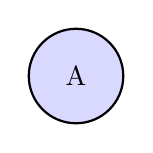
\begin{tikzpicture}
            \draw[thick, fill=blue!15] (0,0) circle (0.6cm);
            \node at (0,0) {A};
        \end{tikzpicture}
        \subcaption{パターンA}
        \label{fig:sub-a}
    \end{subfigure}
    \hfill
    \begin{subfigure}[b]{0.3\columnwidth}
        \centering
        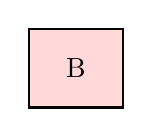
\begin{tikzpicture}
            \draw[thick, fill=red!15] (0,0) rectangle (1.2,1.0);
            \node at (0.6,0.5) {B};
        \end{tikzpicture}
        \subcaption{パターンB}
        \label{fig:sub-b}
    \end{subfigure}
    \hfill
    \begin{subfigure}[b]{0.3\columnwidth}
        \centering
        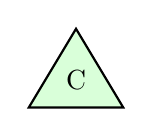
\begin{tikzpicture}
            \draw[thick, fill=green!15] (0,0) -- (1.2,0) -- (0.6,1.0) -- cycle;
            \node at (0.6,0.35) {C};
        \end{tikzpicture}
        \subcaption{パターンC}
        \label{fig:sub-c}
    \end{subfigure}
    \caption{subcaptionによる複数図の例}
    \label{fig:subfigures}
\end{figure}

%% ===========================================================
\section{表の使い方}
\label{sec:table}

表にもキャプションを付け，本文中で必ず参照すること．
表のキャプションは表の上に，図のキャプションは図の下に配置するのが慣例である．
\texttt{booktabs}パッケージの\verb|\toprule|，\verb|\midrule|，\verb|\bottomrule|を使うと見栄えのよい横罫線が引ける．
場合によるが一般的な表であれば縦罫線はあまり使わない方が読みやすい．

表\ref{tab:comparison}に手法の比較表の例を示す．
このように\verb|\multicolumn|を使えばセルの結合ができ，\verb|\cmidrule|で部分的な罫線を引くことができる．

\begin{table}[tb]
    \centering
    \caption{手法の比較}
    \label{tab:comparison}
    \begin{tabular}{lccc}\toprule
        \multirow{2}{*}{手法} & \multicolumn{2}{c}{評価指標} & \multirow{2}{*}{時間 [ms]} \\
        \cmidrule(lr){2-3}
                    & 精度 [\%] & F1値  &       \\ \midrule
        手法A        & 85.2     & 0.83 & 120   \\
        手法B        & 91.7     & 0.90 & 340   \\
        提案手法      & \textbf{93.4} & \textbf{0.92} & 150 \\ \bottomrule
    \end{tabular}
\end{table}

表\ref{tab:schedule}にシンプルな表の例を示す．

\begin{table}[tb]
    \centering
    \caption{卒論卒制スケジュール}
    \label{tab:schedule}
    \begin{tabular}{ll}\toprule
        項目       & 締切日  \\ \midrule
        レジュメ提出 & *月**日 \\
        卒業論文提出 & *月**日 \\
        発表会     & *月**日 \\ \bottomrule
    \end{tabular}
\end{table}

%% ===========================================================
\section{数式の記述}
\label{sec:math}

数式を文中に埋め込む場合は$y = ax + b$のように記述する．
独立した数式には\texttt{equation}環境を用いる．
式(\ref{eq:softmax})にソフトマックス関数の例を示す．
ここで$z_i$は$i$番目のクラスのスコア，$K$はクラスの総数を表す．
このように，数式中の変数や記号は本文中で必ずその意味を説明すること．
\begin{equation}
    \label{eq:softmax}
    \mathrm{softmax}(z_i) = \frac{e^{z_i}}{\sum_{j=1}^{K} e^{z_j}}
\end{equation}
複数行の数式には\texttt{align}環境が使える．
なお，別組の数式に\verb|$$|〜\verb|$$|は使用せず，\verb|\[|〜\verb|\]|または\texttt{equation}環境を用いること．

%% ===========================================================
\section{ソースコードの掲載}
\label{sec:code}

ソースコードを掲載する場合は\texttt{listings}環境を用いると良い．
ソースコード\ref{lst:hello}に例を示す．
\texttt{language}オプションでC，Python，Javaなど言語を切り替えることができ，キーワードや文字列に自動で色が付く．
コードを掲載する際は，論文の主張に関係する部分のみを抜粋すること．

\begin{lstlisting}[caption={Hello Worldの例}, label={lst:hello}, language=c, float=tb]
#include <stdio.h>
// Hello Worldを出力する簡単なCプログラム
int main(void) {
    printf("Hello, World!\n");
    return 0;
}
\end{lstlisting}

%% ===========================================================
\section{参考文献について}
\label{sec:reference}

参考文献リストには，原則として本文中で引用した文献のみを列挙する．
本文中で引用する際には必ず\verb|\cite{}|を用いる．
逆に，他者の研究成果や主張を引用する際に出典を明記しないことは許されない．
十分な参考文献の調査と引用は，研究の新規性の主張に欠かせない．
以下の点にも注意すること．
\begin{itemize}
    \item 参考文献が自分のものばかりになっていないか確認する
    \item 適切な文献が引用されており，その数も十分であること
    \item 既発表の論文等との間に不適切な重複がないこと
\end{itemize}

参考文献の種類ごとの記述例を以下に示す．
\begin{itemize}
    \item \textbf{論文誌}：著者名, ``タイトル'', 誌名, 巻, 号, ページ, 年\cite{lamport}
    \item \textbf{書籍}：著者名, ``書名'', 出版社, 年\cite{tex}
    \item \textbf{Web}：著者名, ``タイトル'', URL, 参照日\cite{ipsj-sample}
\end{itemize}
Webページを参照する場合は最終アクセス日を記載する．
Webページは削除や変更の可能性があるため，可能な限り論文誌や書籍を優先して引用すること．

\LaTeX では\texttt{thebibliography}環境を用いて参考文献リストを記述する．
\verb|\bibitem{キー}|で各文献にキーを割り当て，本文中で\verb|\cite{キー}|と書くことで番号が自動的に振られる．
\begin{lstlisting}[language={[LaTeX]TeX}, numbers=none, frame=single]
\begin{thebibliography}{9}
\bibitem{lamport}
L. Lamport, ``\LaTeX: A Document ...'', 1994.
\end{thebibliography}
\end{lstlisting}
引数の\texttt{9}は文献番号の最大桁数の目安である（10件以上なら\texttt{99}とするがレジュメでそれほど多くの文献を載せることはまずない）．

参考文献にURLを含める場合は，\verb|\url{}|コマンドを使用すること．
\verb|\url{}|を使うと自動で等幅フォントになり，適切な位置で改行される．
直接URLを書いた場合との違いを以下に示す．
\begin{itemize}
    \item \verb|\url{}|あり：\url{https://www.ipsj.or.jp/journal/submit/style.html}
    \item \verb|\url{}|なし：https://www.ipsj.or.jp/journal/submit/style.html
\end{itemize}
\verb|\url{}|を使わないとURLが途中で改行されず，overfullの原因になったり，見た目が崩れることがある．

%% ===========================================================
\section{Overfullへの対処}
\label{sec:overfull}

組版時にoverfull（行がはみ出す現象）を起こさないことが原則である．
提出するソースが自分の環境でoverfullを起こさないよう，文章を工夫する努力を払うこと．
ただし，\texttt{flushleft}環境や\verb|\\|，\verb|\linebreak|による両端揃えをしない形での回避はできるだけ避ける．
overfullが発生しやすい例として，文中の長い数式，\verb|\verb|コマンド，長い英単語がある．
これらを段落の先頭付近に置かないようにするだけでも改善できることが多い．

%% ===========================================================
\section{PDF提出時の注意}
\label{sec:pdf}

提出前には以下の点を最終確認すること．
後の修正の手間を最小にするために，この段階で記述の誤りを完全に除去するよう綿密にチェックすること\cite{ipsj-sample}．
\begin{itemize}
    \item \verb|\ThisIsDraft|が削除またはコメントアウトされているか
    \item タイトルが卒業論文と一致しているか
    \item 学籍番号・氏名・指導教員名に誤りがないか
    \item 図表番号・参考文献番号が正しく参照されているか
    \item 参考文献に未参照のものがないか
    \item フォントが埋め込まれているか（印刷時の文字化けを防ぐ）
    \item overfullが発生していないか
\end{itemize}

%% ===========================================================
\section{おわりに}
\label{sec:conclusion}

本テンプレートの使い方と，卒業研究・卒業制作それぞれのレジュメ執筆時の注意点を示した．
レジュメは学科全体で取りまとめられ，全研究室に配布される．
教員や同級生だけでなく，今後の全ての後輩たちが目にするものである．
内容・体裁ともにしっかりした原稿を作成してほしい．

\begin{thebibliography}{9}
\bibitem{lamport}
L. Lamport, ``\LaTeX: A Document Preparation System'', Addison-Wesley, 2nd edition, 1994.

\bibitem{tex}
奥村晴彦, 黒木祐介, ``改訂第9版 \LaTeX2$\epsilon$ 美文書作成入門'', 技術評論社, 2023.

\bibitem{kisaragi}
木下是雄, ``理科系の作文技術'', 中公新書, 1981.

\bibitem{ipsj-sample}
情報処理学会論文誌ジャーナル編集委員会, ``情報処理学会論文誌ジャーナル論文の準備方法'', \url{https://www.ipsj.or.jp/journal/submit/style.html}, 参照 2026-01-15.

\end{thebibliography}

    % 
% ----------
\title{タイトル} % タイトル

\author{%
    X12345 あなたの名前
}

\supervisor{教員名}

% ----------

\maketitle

%% ===========================================================
\section{はじめに}
あのイーハトーヴォのすきとおった風，夏でも底に冷たさをもつ青いそら，うつくしい森で飾られたモリーオ市，郊外のぎらぎらひかる草の波．またそのなかでいっしょになったたくさんのひとたち，ファゼーロとロザーロ，羊飼のミーロや，顔の赤いこどもたち，地主のテーモ，山猫博士のボーガント・デストゥパーゴなど，いまこの暗い巨きな石の建物のなかで考えていると，みんなむかし風のなつかしい青い幻燈のように思われます．では，わたくしはいつかの小さなみだしをつけながら，しずかにあの年のイーハトーヴォの五月から十月までを書きつけましょう．

\section{関連研究・事例}
あのイーハトーヴォのすきとおった風，夏でも底に冷たさをもつ青いそら，うつくしい森で飾られたモリーオ市，郊外のぎらぎらひかる草の波．またそのなかでいっしょになったたくさんのひとたち，ファゼーロとロザーロ，羊飼のミーロや，顔の赤いこどもたち，地主のテーモ，山猫博士のボーガント・デストゥパーゴなど，いまこの暗い巨きな石の建物のなかで考えていると，みんなむかし風のなつかしい青い幻燈のように思われます．では，わたくしはいつかの小さなみだしをつけながら，しずかにあの年のイーハトーヴォの五月から十月までを書きつけましょう．

\section{提案手法}
あのイーハトーヴォのすきとおった風，夏でも底に冷たさをもつ青いそら，うつくしい森で飾られたモリーオ市，郊外のぎらぎらひかる草の波．またそのなかでいっしょになったたくさんのひとたち，ファゼーロとロザーロ，羊飼のミーロや，顔の赤いこどもたち，地主のテーモ，山猫博士のボーガント・デストゥパーゴなど，いまこの暗い巨きな石の建物のなかで考えていると，みんなむかし風のなつかしい青い幻燈のように思われます．では，わたくしはいつかの小さなみだしをつけながら，しずかにあの年のイーハトーヴォの五月から十月までを書きつけましょう．

\section{実験・評価}
あのイーハトーヴォのすきとおった風，夏でも底に冷たさをもつ青いそら，うつくしい森で飾られたモリーオ市，郊外のぎらぎらひかる草の波．またそのなかでいっしょになったたくさんのひとたち，ファゼーロとロザーロ，羊飼のミーロや，顔の赤いこどもたち，地主のテーモ，山猫博士のボーガント・デストゥパーゴなど，いまこの暗い巨きな石の建物のなかで考えていると，みんなむかし風のなつかしい青い幻燈のように思われます．では，わたくしはいつかの小さなみだしをつけながら，しずかにあの年のイーハトーヴォの五月から十月までを書きつけましょう．

\section{おわりに}
あのイーハトーヴォのすきとおった風，夏でも底に冷たさをもつ青いそら，うつくしい森で飾られたモリーオ市，郊外のぎらぎらひかる草の波．またそのなかでいっしょになったたくさんのひとたち，ファゼーロとロザーロ，羊飼のミーロや，顔の赤いこどもたち，地主のテーモ，山猫博士のボーガント・デストゥパーゴなど，いまこの暗い巨きな石の建物のなかで考えていると，みんなむかし風のなつかしい青い幻燈のように思われます．では，わたくしはいつかの小さなみだしをつけながら，しずかにあの年のイーハトーヴォの五月から十月までを書きつけましょう．

\begin{thebibliography}{9}
\bibitem{label-1}
参考文献の例1, 著者名, ``タイトル'', 出版社, 年.
\bibitem{label-2}
著者名, ``タイトル'', 論文誌, No.X, pp.0-1, (年)
\bibitem{label-3}
参考文献の例1, 著者名, ``タイトル'', \url{https://example.com}
\end{thebibliography}
    
\end{document}
